% !TEX root = ../masterthesis.tex
\chapter{Methods}

\section{Setup}

The setup used for the measurements described in following chapters is sketched in figure~\ref{fig:setupflat}.

\begin{figure}[H]
	\centering
	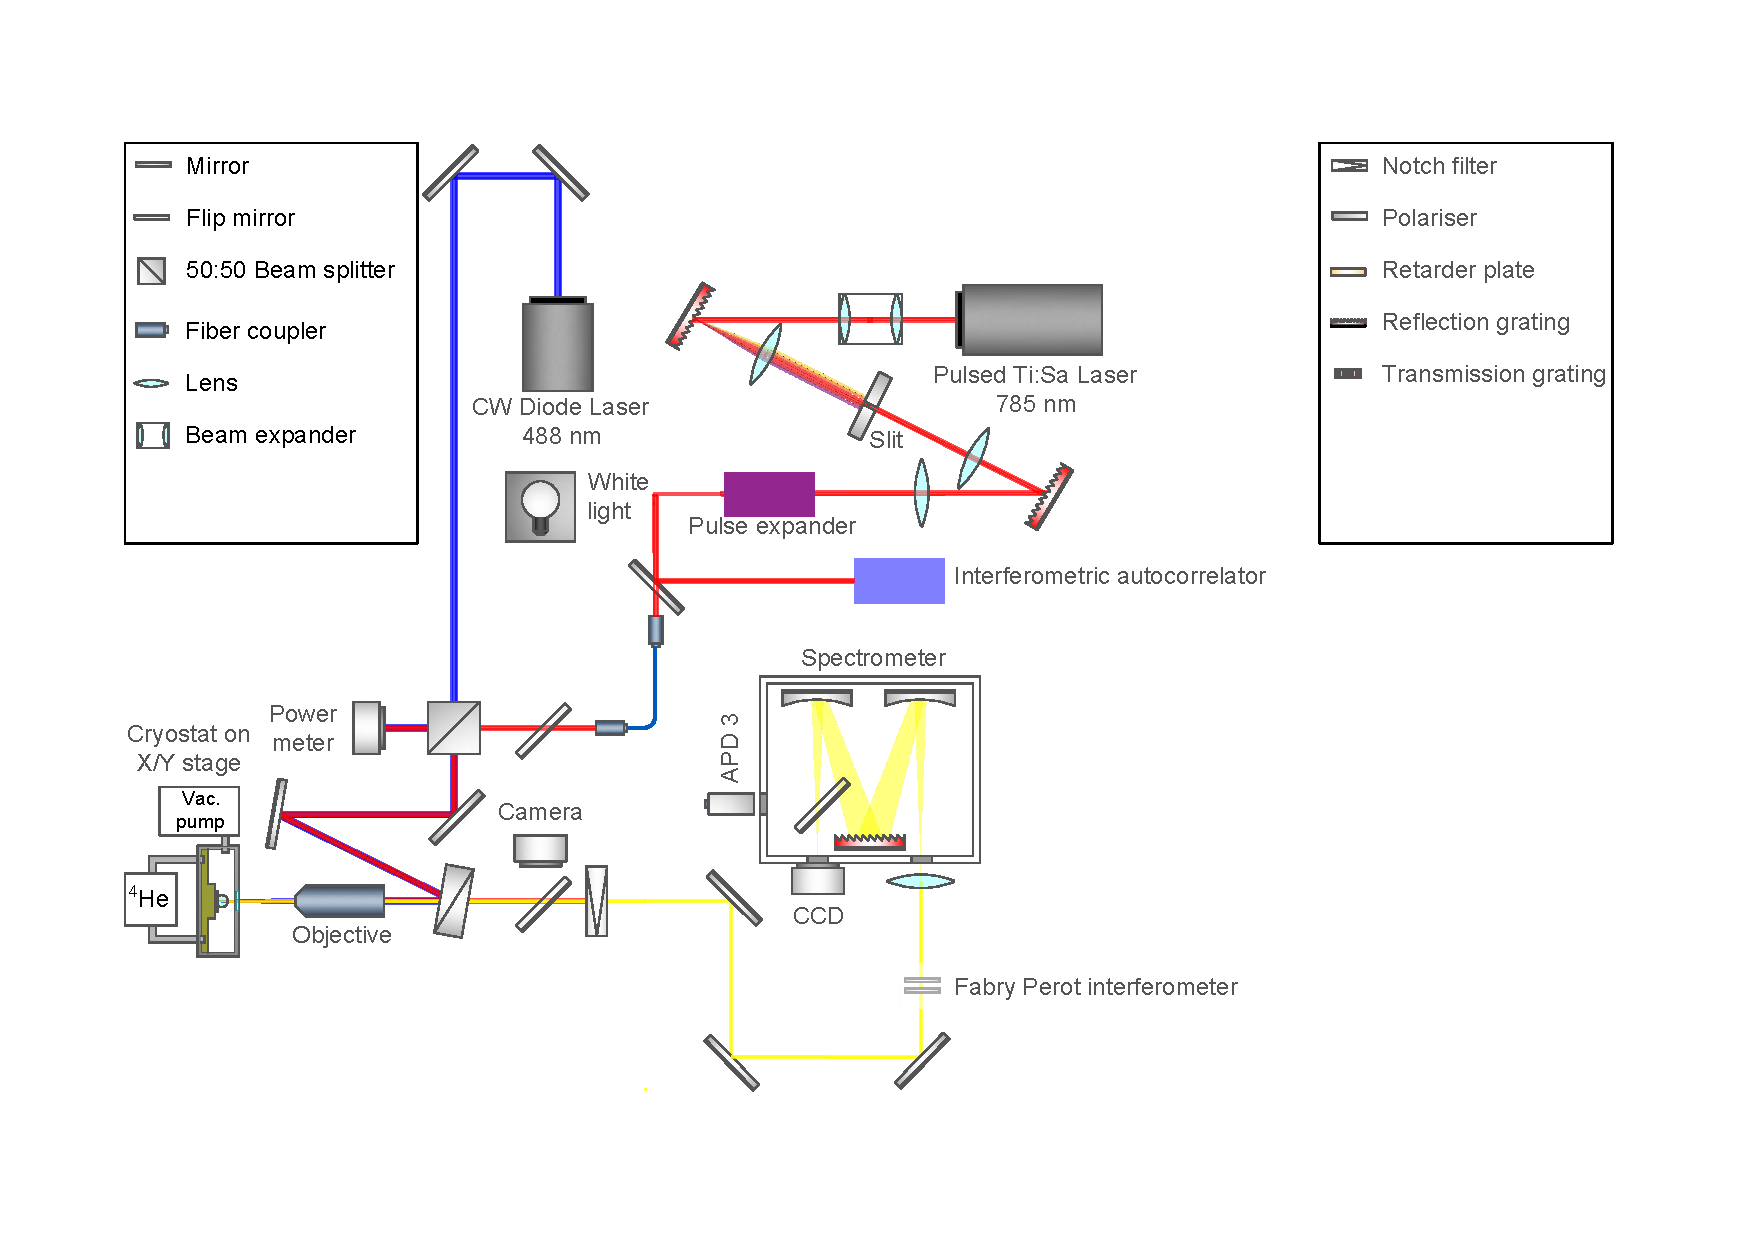
\includegraphics[width=\linewidth]{figures/setup/Setup_flat}
	\caption[Complete experimental setup]{Complete experimental setup, which was used in order to quantify the chirp of the Ti:Sa Laser and resolve spectral emission of a quantum dot~\cite{schimpf_towards_2017}.}
	\label{fig:setupflat}
\end{figure}

\todo{Introduce a chapter "Methods" (I would say between chapter QDs and ARP) and decribe some basics how you measure stuff, such as micro-PL, the cryostat etc}